\section{Exercício 1}
\begin{figure}[H]
    \centering
    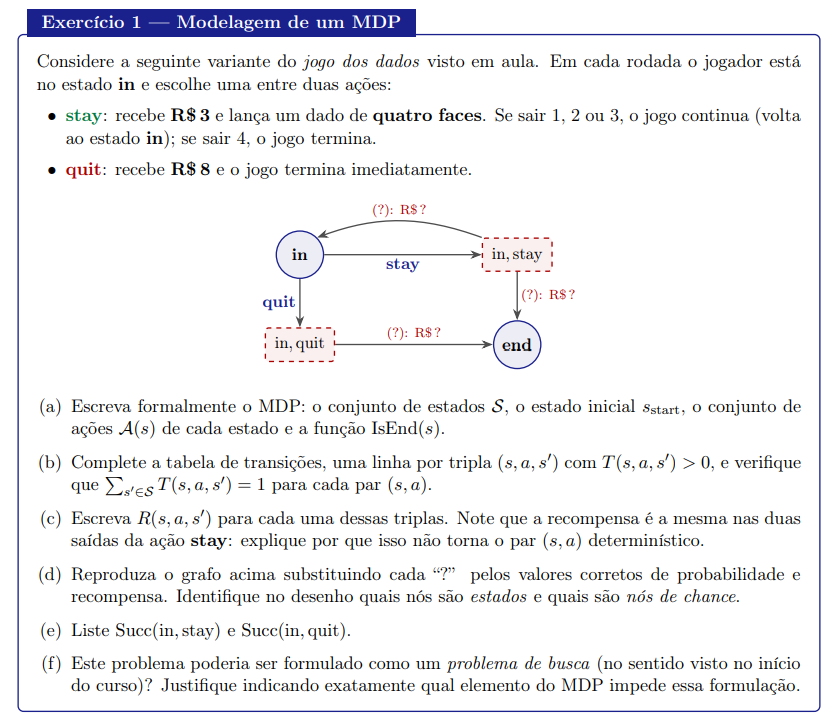
\includegraphics[width=0.8\textwidth]{ex1.png}
    \label{fig:ex1}
\end{figure}

\subsection{Item (a)}

O Processo de Decisão de Markov (MDP) pode ser definido
formalmente pelos seguintes elementos:

\begin{itemize}
    \item \textbf{Conjunto de estados:}
    \[
        S = \{in, end\}
    \]
    em que $in$ representa o jogo em andamento e
    $end$ representa o estado terminal.

    \item \textbf{Estado inicial:}
    \[
        s_{\text{start}} = in
    \]

    \item \textbf{Conjunto de ações disponíveis:}
    \[
        A(s) =
        \begin{cases}
            \{stay, quit\}, & \text{se } s = in,\\
            \emptyset, & \text{se } s = end.
        \end{cases}
    \]

    \item \textbf{Função de identificação do estado terminal:}
    \[
        IsEnd(s) =
        \begin{cases}
            \text{True}, & \text{se } s = end,\\
            \text{False}, & \text{se } s = in.
        \end{cases}
    \]
\end{itemize}


\subsection{Item (b)}

A função de transição $T(s,a,s')$ representa a
probabilidade de alcançar o estado $s'$ ao executar
a ação $a$ no estado $s$.

As transições possíveis são apresentadas na
Tabela~\ref{tab:transicoes_mdp}.

\begin{table}[H]
    \centering
    \caption{Probabilidades de transição do MDP}
    \label{tab:transicoes_mdp}
    \begin{tabular}{cccc}
        \toprule
        $s$ & $a$ & $s'$ & $T(s,a,s')$ \\
        \midrule
        $in$ & $stay$ & $in$  & $\frac{3}{4}$ \\
        $in$ & $stay$ & $end$ & $\frac{1}{4}$ \\
        $in$ & $quit$ & $end$ & $1$ \\
        \bottomrule
    \end{tabular}
\end{table}

Para verificar a validade das probabilidades,
devemos garantir que:

\[
    \sum_{s' \in S} T(s,a,s') = 1
\]

para cada par $(s,a)$ com ação disponível.

\textbf{Ação stay:}

Como três das quatro faces do dado mantêm o
jogador no estado $in$ e uma encerra o jogo:

\[
\begin{aligned}
    \sum_{s' \in S} T(in,stay,s')
    &= T(in,stay,in) + T(in,stay,end)\\
    &= \frac{3}{4} + \frac{1}{4}\\
    &= 1.
\end{aligned}
\]

\textbf{Ação quit:}

Como a ação $quit$ encerra o jogo imediatamente:

\[
\begin{aligned}
    \sum_{s' \in S} T(in,quit,s')
    &= T(in,quit,in) + T(in,quit,end)\\
    &= 0 + 1\\
    &= 1.
\end{aligned}
\]

Portanto, todas as distribuições de probabilidade
de transição são válidas, pois suas probabilidades
somam $1$ para cada par estado-ação.


\subsection{Item (c)}

A função de recompensa $R(s,a,s')$ representa
a recompensa recebida ao executar a ação $a$
no estado $s$ e alcançar o estado $s'$.

As recompensas das transições são:

\[
\begin{aligned}
    R(in,stay,in) &= 3,\\
    R(in,stay,end) &= 3,\\
    R(in,quit,end) &= 8.
\end{aligned}
\]

A ação $stay$ fornece uma recompensa de R\$ 3,
independentemente do resultado do lançamento do dado.
Por outro lado, a ação $quit$ fornece uma recompensa
de R\$ 8 e encerra imediatamente o jogo.

Embora a recompensa da ação $stay$ seja sempre
a mesma, isso não torna o par $(in,stay)$
determinístico, pois existem dois estados sucessores
possíveis:

\[
    T(in,stay,in) = \frac{3}{4}
\]

\[
    T(in,stay,end) = \frac{1}{4}
\]

Portanto, a recompensa da ação $stay$ é
determinística, mas a transição de estados é
estocástica, uma vez que o próximo estado depende
do resultado aleatório do lançamento do dado.

\subsection{Item (d)}

O grafo do MDP é apresentado na
Figura~\ref{fig:grafo_mdp}, com as probabilidades
de transição e suas respectivas recompensas.

\begin{figure}[H]
    \centering

    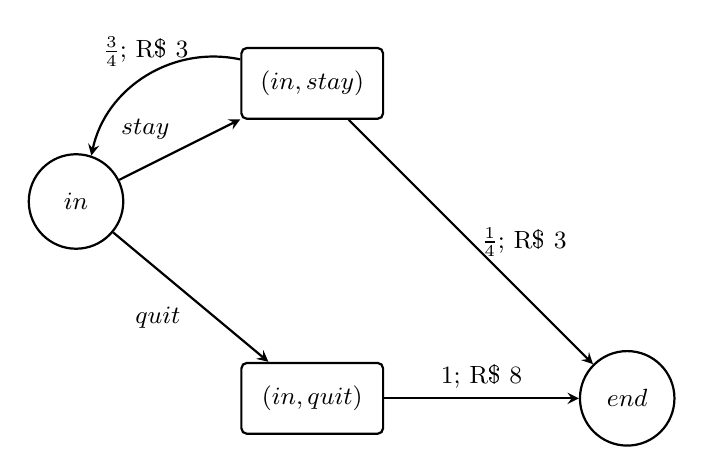
\begin{tikzpicture}[
        >=stealth,
        state/.style={
            circle,
            draw,
            minimum size=1.2cm,
            thick
        },
        chance/.style={
            rectangle,
            draw,
            rounded corners=2pt,
            minimum width=1.8cm,
            minimum height=0.9cm,
            thick
        },
        every node/.style={font=\small}
    ]

    % Nos de estado
    \node[state] (in) at (0,0) {$in$};
    \node[state] (end) at (7,-2.5) {$end$};

    % Nos de chance
    \node[chance] (stay) at (3,1.5) {$(in,stay)$};
    \node[chance] (quit) at (3,-2.5) {$(in,quit)$};

    % Escolha das acoes
    \draw[->,thick]
        (in) -- node[above left] {$stay$} (stay);

    \draw[->,thick]
        (in) -- node[below left] {$quit$} (quit);

    % Transicao stay para in
    \draw[->,thick]
        (stay) to[bend right=45]
        node[above] {$\frac{3}{4}$; R\$ 3} (in);

    % Transicao stay para end
    \draw[->,thick]
        (stay) -- node[right] {$\frac{1}{4}$; R\$ 3} (end);

    % Transicao quit para end
    \draw[->,thick]
        (quit) -- node[above] {$1$; R\$ 8} (end);

    \end{tikzpicture}

    \caption{Grafo do MDP com probabilidades
    de transição e recompensas.}
    \label{fig:grafo_mdp}
\end{figure}

No grafo, os nós circulares representam os
\textbf{estados} do MDP ($in$ e $end$), enquanto
os nós retangulares representam os
\textbf{nós de chance} associados aos pares
estado-ação $(in,stay)$ e $(in,quit)$.

A partir do estado $in$, o jogador escolhe
entre as ações $stay$ e $quit$.

Ao escolher $stay$, recebe R\$ 3 e pode retornar
ao estado $in$ com probabilidade $\frac{3}{4}$,
ou alcançar o estado terminal $end$ com
probabilidade $\frac{1}{4}$.

Ao escolher $quit$, recebe R\$ 8 e alcança
o estado terminal $end$ com probabilidade $1$.

\subsection{Item (e)}

O conjunto de estados sucessores $Succ(s,a)$
contém todos os estados que podem ser alcançados
a partir do estado $s$ após executar a ação $a$,
com probabilidade de transição maior que zero.

Para a ação $stay$, o jogador pode permanecer
no estado $in$, com probabilidade $\frac{3}{4}$,
ou alcançar o estado terminal $end$, com
probabilidade $\frac{1}{4}$. Portanto:

\[
    Succ(in,stay) = \{in,end\}
\]

Para a ação $quit$, o jogo termina imediatamente,
de modo que o único estado sucessor possível
é $end$. Assim:

\[
    Succ(in,quit) = \{end\}
\]


\subsection{Item (f)}

O problema não pode ser formulado diretamente
como um problema de busca tradicional determinística,
pois apresenta transições estocásticas.

Em um problema de busca determinística, a função
de transição associa cada par estado-ação $(s,a)$
a um único estado sucessor $s'$.

Entretanto, no MDP apresentado, a ação $stay$
possui dois resultados possíveis:

\[
    T(in,stay,in) = \frac{3}{4}
\]

\[
    T(in,stay,end) = \frac{1}{4}
\]

Assim, o próximo estado não é determinado
exclusivamente pela ação escolhida, mas também
pelo resultado aleatório do lançamento do dado.

Portanto, o elemento que impede a formulação
direta como um problema de busca determinística
é a \textbf{função de transição probabilística}
$T(s,a,s')$, que permite múltiplos estados
sucessores para um mesmo par estado-ação.

Nesse caso, a modelagem como MDP é mais adequada,
pois permite representar tanto as probabilidades
de transição quanto as recompensas associadas
às decisões.

\section{Exercício 2}
\begin{figure}[H]
    \centering
    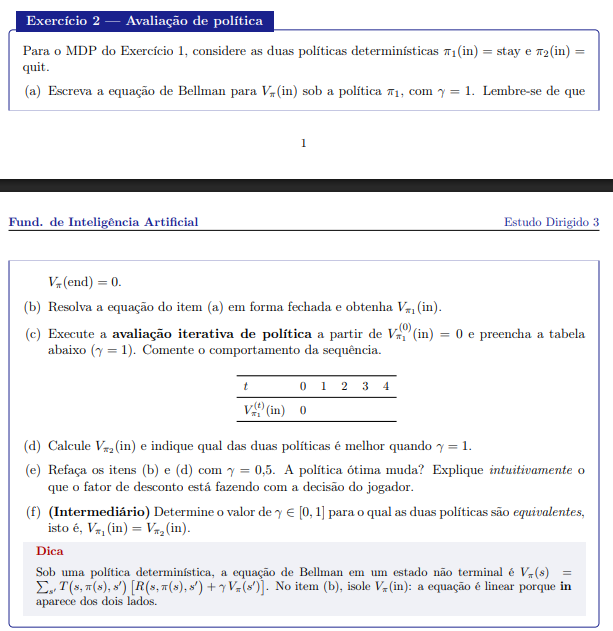
\includegraphics[width=0.8\textwidth]{ex2.png}
    \label{fig:ex2}
\end{figure}


\subsection{Item (a)}

Considere a política determinística $\pi_1$,
na qual o jogador sempre escolhe a ação $stay$:

\[
    \pi_1(in) = stay
\]

A equação de Bellman para avaliação de uma
política $\pi$ é dada por:

\[
    V_{\pi}(s) =
    \sum_{s' \in S} T(s,\pi(s),s')
    \left[
        R(s,\pi(s),s') + \gamma V_{\pi}(s')
    \right]
\]

Para a política $\pi_1$, considerando $\gamma = 1$
e $V_{\pi_1}(end) = 0$, temos:

\[
\begin{aligned}
    V_{\pi_1}(in)
    &= \frac{3}{4}
    \left[3 + V_{\pi_1}(in)\right]
    + \frac{1}{4}
    \left[3 + V_{\pi_1}(end)\right]
    \\[6pt]
    &= \frac{3}{4}
    \left[3 + V_{\pi_1}(in)\right]
    + \frac{1}{4}(3 + 0)
    \\[6pt]
    &= \frac{9}{4}
    + \frac{3}{4}V_{\pi_1}(in)
    + \frac{3}{4}
\end{aligned}
\]

Portanto, a equação de Bellman para a
política $\pi_1$ é:

\[
    \boxed{
        V_{\pi_1}(in) =
        3 + \frac{3}{4}V_{\pi_1}(in)
    }
\]


\subsection{Item (b)}

A partir da equação de Bellman obtida no item (a),
temos:

\[
    V_{\pi_1}(in) =
    3 + \frac{3}{4}V_{\pi_1}(in)
\]

Isolando $V_{\pi_1}(in)$:

\[
\begin{aligned}
    V_{\pi_1}(in)
    - \frac{3}{4}V_{\pi_1}(in) &= 3
    \\[6pt]
    \left(1-\frac{3}{4}\right)V_{\pi_1}(in) &= 3
    \\[6pt]
    \frac{1}{4}V_{\pi_1}(in) &= 3
    \\[6pt]
    V_{\pi_1}(in) &= \frac{3}{1/4}
\end{aligned}
\]

Portanto:

\[
    \boxed{V_{\pi_1}(in) = 12}
\]

Assim, seguindo a política $\pi_1$, na qual o
jogador sempre escolhe a ação $stay$, a recompensa
total esperada é de R\$ 12,00.

Esse resultado considera todas as rodadas
possíveis até o encerramento do jogo,
com fator de desconto $\gamma = 1$.


\subsection{Item (c)}

A avaliação iterativa da política $\pi_1$ é
realizada a partir do valor inicial:

\[
    V_{\pi_1}^{(0)}(in) = 0
\]

Considerando $\gamma = 1$, a equação
de atualização é:

\[
    V_{\pi_1}^{(t+1)}(in) =
    3 + \frac{3}{4}V_{\pi_1}^{(t)}(in)
\]

Aplicando a equação sucessivamente:

\[
\begin{aligned}
    V_{\pi_1}^{(1)}(in)
    &= 3 + \frac{3}{4}(0) = 3
    \\[6pt]
    V_{\pi_1}^{(2)}(in)
    &= 3 + \frac{3}{4}(3) = 5{,}25
    \\[6pt]
    V_{\pi_1}^{(3)}(in)
    &= 3 + \frac{3}{4}(5{,}25) = 6{,}9375
    \\[6pt]
    V_{\pi_1}^{(4)}(in)
    &= 3 + \frac{3}{4}(6{,}9375)
    = 8{,}203125
\end{aligned}
\]

Os resultados são apresentados na
Tabela~\ref{tab:avaliacao_politica}.

\begin{table}[H]
    \centering
    \caption{Avaliação iterativa da política $\pi_1$}
    \label{tab:avaliacao_politica}
    \begin{tabular}{cccccc}
        \toprule
        $t$ & 0 & 1 & 2 & 3 & 4 \\
        \midrule
        $V_{\pi_1}^{(t)}(in)$
        & 0 & 3 & 5,25 & 6,9375 & 8,203125 \\
        \bottomrule
    \end{tabular}
\end{table}

Observa-se que a sequência de valores é
monotonicamente crescente, aproximando-se
progressivamente do valor exato obtido
no item (b):

\[
    \lim_{t \to \infty} V_{\pi_1}^{(t)}(in) = 12
\]

A convergência ocorre porque, a cada iteração,
a diferença em relação ao valor exato é
multiplicada por $\frac{3}{4}$, tornando-se
progressivamente menor.


\subsection{Item (d)}

Considere a política determinística $\pi_2$,
na qual o jogador sempre escolhe a ação $quit$:

\[
    \pi_2(in) = quit
\]

Pela equação de Bellman, considerando
$\gamma = 1$, temos:

\[
\begin{aligned}
    V_{\pi_2}(in)
    &= T(in,quit,end)
    \left[
        R(in,quit,end) + V_{\pi_2}(end)
    \right]
    \\[6pt]
    &= 1 \cdot (8 + 0)
    \\[6pt]
    &= 8
\end{aligned}
\]

Portanto:

\[
    \boxed{V_{\pi_2}(in) = 8}
\]

Comparando os valores das duas políticas:

\[
\begin{aligned}
    V_{\pi_1}(in) &= 12\\
    V_{\pi_2}(in) &= 8
\end{aligned}
\]

Como:

\[
    V_{\pi_1}(in) > V_{\pi_2}(in)
\]

conclui-se que a política $\pi_1$, que sempre
escolhe a ação $stay$, é a melhor para
$\gamma = 1$.

Isso ocorre porque a possibilidade de continuar
recebendo recompensas de R\$ 3 nas rodadas
seguintes resulta em uma recompensa total
esperada de R\$ 12, superior aos R\$ 8
recebidos imediatamente pela ação $quit$.


\subsection{Item (e)}

Considerando o fator de desconto $\gamma = 0{,}5$,
recalculamos os valores das políticas $\pi_1$
e $\pi_2$.

\textbf{Política $\pi_1(in) = stay$:}

Pela equação de Bellman:

\[
\begin{aligned}
    V_{\pi_1}(in)
    &= \frac{3}{4}
    \left[3 + 0{,}5V_{\pi_1}(in)\right]
    + \frac{1}{4}(3 + 0)
    \\[6pt]
    &= 3 + 0{,}375V_{\pi_1}(in)
\end{aligned}
\]

Isolando $V_{\pi_1}(in)$:

\[
\begin{aligned}
    V_{\pi_1}(in) - 0{,}375V_{\pi_1}(in) &= 3
    \\[6pt]
    0{,}625V_{\pi_1}(in) &= 3
    \\[6pt]
    V_{\pi_1}(in) &= \frac{3}{0{,}625}
    \\[6pt]
    &= 4{,}8
\end{aligned}
\]

Portanto:

\[
    \boxed{V_{\pi_1}(in) = 4{,}8}
\]

\textbf{Política $\pi_2(in) = quit$:}

Como a ação $quit$ encerra imediatamente o jogo,
não existem recompensas futuras a serem descontadas.

\[
\begin{aligned}
    V_{\pi_2}(in)
    &= 1 \cdot \left[8 + 0{,}5(0)\right]
    \\[6pt]
    &= 8
\end{aligned}
\]

Portanto:

\[
    \boxed{V_{\pi_2}(in) = 8}
\]

\textbf{Comparação das políticas:}

\[
    V_{\pi_2}(in) = 8 > 4{,}8 = V_{\pi_1}(in)
\]

Logo, a política ótima muda de $stay$ para $quit$
quando o fator de desconto passa de $\gamma = 1$
para $\gamma = 0{,}5$.

Isso ocorre porque o fator de desconto reduz
a importância das recompensas futuras em relação
às recompensas imediatas.

Com $\gamma = 1$, todas as recompensas possuem
o mesmo peso, independentemente de quando são
recebidas, favorecendo a ação $stay$.

Já com $\gamma = 0{,}5$, as recompensas futuras
perdem valor progressivamente, tornando mais
vantajoso receber R\$ 8 imediatamente por meio
da ação $quit$.


\subsection{Item (f)}

Para determinar o fator de desconto $\gamma$
que torna as duas políticas equivalentes,
devemos encontrar o valor que satisfaz:

\[
    V_{\pi_1}(in) = V_{\pi_2}(in)
\]

\textbf{Política $\pi_1(in) = stay$:}

Aplicando a equação de Bellman para um
fator de desconto genérico $\gamma$:

\[
\begin{aligned}
    V_{\pi_1}(in)
    &= \frac{3}{4}
    \left[3 + \gamma V_{\pi_1}(in)\right]
    + \frac{1}{4}(3 + 0)
    \\[6pt]
    &= 3 + \frac{3}{4}\gamma V_{\pi_1}(in)
\end{aligned}
\]

Isolando $V_{\pi_1}(in)$:

\[
\begin{aligned}
    V_{\pi_1}(in)
    - \frac{3}{4}\gamma V_{\pi_1}(in) &= 3
    \\[6pt]
    V_{\pi_1}(in)
    \left(1-\frac{3}{4}\gamma\right) &= 3
\end{aligned}
\]

Portanto:

\[
    V_{\pi_1}(in) =
    \frac{3}{1-\frac{3}{4}\gamma}
\]

\textbf{Política $\pi_2(in) = quit$:}

Como a ação $quit$ encerra imediatamente o jogo:

\[
    V_{\pi_2}(in) = 8
\]

\textbf{Igualando os valores das políticas:}

\[
\begin{aligned}
    \frac{3}{1-\frac{3}{4}\gamma} &= 8
    \\[6pt]
    3 &= 8\left(1-\frac{3}{4}\gamma\right)
    \\[6pt]
    3 &= 8 - 6\gamma
    \\[6pt]
    6\gamma &= 5
    \\[6pt]
    \gamma &= \frac{5}{6}
\end{aligned}
\]

Assim, o fator de desconto que torna as
duas políticas equivalentes é:

\[
    \boxed{\gamma = \frac{5}{6} \approx 0{,}8333}
\]

Nesse ponto, ambas as políticas apresentam
a mesma recompensa total esperada de R\$ 8.

Para $\gamma < \frac{5}{6}$, a política $quit$
é mais vantajosa, enquanto para
$\gamma > \frac{5}{6}$, a política $stay$
apresenta maior valor esperado.

\section{Exercício 3}
\begin{figure}[H]
    \centering
    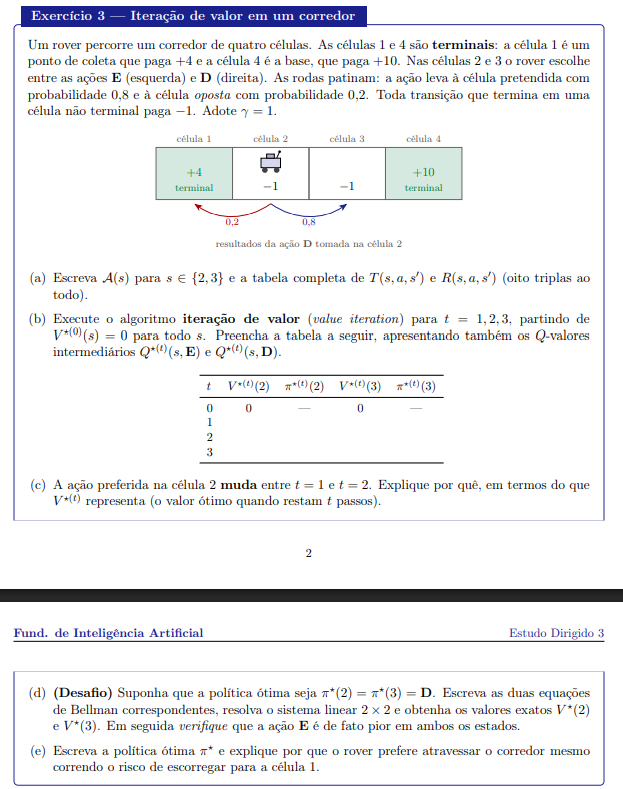
\includegraphics[width=0.8\textwidth]{ex3.png}
    \label{fig:ex3}
\end{figure}



\subsection{Item (a)}

O conjunto de estados do MDP é dado por:

\[
    S = \{1,2,3,4\}
\]

As células $1$ e $4$ são estados terminais,
enquanto as células $2$ e $3$ permitem
a escolha entre as ações $E$ (esquerda)
e $D$ (direita).

Assim, os conjuntos de ações disponíveis são:

\[
    A(2) = A(3) = \{E,D\}
\]

As probabilidades de transição dependem
do movimento escolhido pelo rover.
A direção pretendida ocorre com probabilidade
$0{,}8$, enquanto o movimento na direção
oposta ocorre com probabilidade $0{,}2$.

As recompensas são determinadas pelo
estado de destino:

\[
    R(s,a,s') =
    \begin{cases}
        +4, & \text{se } s'=1,\\
        -1, & \text{se } s'\in\{2,3\},\\
        +10, & \text{se } s'=4.
    \end{cases}
\]

A Tabela~\ref{tab:transicoes_rover} apresenta
as oito transições possíveis do MDP.

\begin{table}[H]
    \centering
    \caption{Transições e recompensas do rover}
    \label{tab:transicoes_rover}
    \begin{tabular}{ccccc}
        \toprule
        $s$ & $a$ & $s'$ & $T(s,a,s')$ & $R(s,a,s')$ \\
        \midrule
        2 & E & 1 & $0{,}8$ & $+4$ \\
        2 & E & 3 & $0{,}2$ & $-1$ \\
        2 & D & 3 & $0{,}8$ & $-1$ \\
        2 & D & 1 & $0{,}2$ & $+4$ \\
        \midrule
        3 & E & 2 & $0{,}8$ & $-1$ \\
        3 & E & 4 & $0{,}2$ & $+10$ \\
        3 & D & 4 & $0{,}8$ & $+10$ \\
        3 & D & 2 & $0{,}2$ & $-1$ \\
        \bottomrule
    \end{tabular}
\end{table}

Para cada par estado-ação $(s,a)$,
a soma das probabilidades das transições
possíveis é igual a $1$:

\[
    \sum_{s'\in S}T(s,a,s')
    = 0{,}8 + 0{,}2 = 1
\]

Portanto, as distribuições de probabilidade
de transição são válidas para todas
as ações disponíveis.


\subsection{Item (b)}

O algoritmo de iteração de valor (\textit{Value Iteration})
calcula iterativamente os valores ótimos dos estados,
considerando as recompensas imediatas e os valores
esperados dos estados sucessores.

A equação de atualização dos Q-valores é:

\[
Q^{\star(t)}(s,a) =
\sum_{s'\in S} T(s,a,s')
\left[R(s,a,s')+\gamma V^{\star(t-1)}(s')\right]
\]

O valor ótimo e a ação escolhida são dados por:

\[
V^{\star(t)}(s) = \max_{a\in A(s)}Q^{\star(t)}(s,a)
\]

\[
\pi^{\star(t)}(s) =
\arg\max_{a\in A(s)}Q^{\star(t)}(s,a)
\]

Consideramos $\gamma=1$ e os valores iniciais:

\[
V^{\star(0)}(s)=0,\quad \forall s\in S
\]

Como as células $1$ e $4$ são terminais,
seus valores permanecem iguais a zero
em todas as iterações.

\subsubsection*{Iteração 1}

Utilizando os valores iniciais iguais a zero:

\textbf{Célula 2:}

\[
\begin{aligned}
Q^{\star(1)}(2,E)
&=0{,}8(4)+0{,}2(-1)\\
&=3
\\[6pt]
Q^{\star(1)}(2,D)
&=0{,}8(-1)+0{,}2(4)\\
&=0
\end{aligned}
\]

Logo:

\[
V^{\star(1)}(2)=3,
\qquad \pi^{\star(1)}(2)=E
\]

\textbf{Célula 3:}

\[
\begin{aligned}
Q^{\star(1)}(3,E)
&=0{,}8(-1)+0{,}2(10)\\
&=1{,}2
\\[6pt]
Q^{\star(1)}(3,D)
&=0{,}8(10)+0{,}2(-1)\\
&=7{,}8
\end{aligned}
\]

Logo:

\[
V^{\star(1)}(3)=7{,}8,
\qquad \pi^{\star(1)}(3)=D
\]

\subsubsection*{Iteração 2}

Utilizando os valores da primeira iteração:

\textbf{Célula 2:}

\[
\begin{aligned}
Q^{\star(2)}(2,E)
&=0{,}8(4)+0{,}2(-1+7{,}8)\\
&=4{,}56
\\[6pt]
Q^{\star(2)}(2,D)
&=0{,}8(-1+7{,}8)+0{,}2(4)\\
&=6{,}24
\end{aligned}
\]

Logo:

\[
V^{\star(2)}(2)=6{,}24,
\qquad \pi^{\star(2)}(2)=D
\]

\textbf{Célula 3:}

\[
\begin{aligned}
Q^{\star(2)}(3,E)
&=0{,}8(-1+3)+0{,}2(10)\\
&=3{,}6
\\[6pt]
Q^{\star(2)}(3,D)
&=0{,}8(10)+0{,}2(-1+3)\\
&=8{,}4
\end{aligned}
\]

Logo:

\[
V^{\star(2)}(3)=8{,}4,
\qquad \pi^{\star(2)}(3)=D
\]

\subsubsection*{Iteração 3}

Utilizando os valores da segunda iteração:

\textbf{Célula 2:}

\[
\begin{aligned}
Q^{\star(3)}(2,E)
&=0{,}8(4)+0{,}2(-1+8{,}4)\\
&=4{,}68
\\[6pt]
Q^{\star(3)}(2,D)
&=0{,}8(-1+8{,}4)+0{,}2(4)\\
&=6{,}72
\end{aligned}
\]

Logo:

\[
V^{\star(3)}(2)=6{,}72,
\qquad \pi^{\star(3)}(2)=D
\]

\textbf{Célula 3:}

\[
\begin{aligned}
Q^{\star(3)}(3,E)
&=0{,}8(-1+6{,}24)+0{,}2(10)\\
&=6{,}192
\\[6pt]
Q^{\star(3)}(3,D)
&=0{,}8(10)+0{,}2(-1+6{,}24)\\
&=9{,}048
\end{aligned}
\]

Logo:

\[
V^{\star(3)}(3)=9{,}048,
\qquad \pi^{\star(3)}(3)=D
\]

\subsubsection*{Tabela de resultados}

A Tabela~\ref{tab:iteracao_valor_rover}
apresenta os valores ótimos e as ações
selecionadas em cada iteração.

\begin{table}[H]
\centering
\caption{Resultados da iteração de valor}
\label{tab:iteracao_valor_rover}
\begin{tabular}{ccccc}
\toprule
$t$ & $V^{\star(t)}(2)$ & $\pi^{\star(t)}(2)$
& $V^{\star(t)}(3)$ & $\pi^{\star(t)}(3)$\\
\midrule
0 & 0 & -- & 0 & --\\
1 & 3 & E & 7,8 & D\\
2 & 6,24 & D & 8,4 & D\\
3 & 6,72 & D & 9,048 & D\\
\bottomrule
\end{tabular}
\end{table}

Observa-se que, na primeira iteração,
a ação preferida na célula $2$ é $E$.
Entretanto, a partir da segunda iteração,
a ação preferida passa a ser $D$.

Isso ocorre porque o algoritmo passa a
considerar as recompensas futuras
associadas aos estados sucessores.


\subsection{Item (c)}

A mudança da ação preferida na célula $2$
ocorre porque $V^{\star(t)}(s)$ representa
a recompensa total esperada máxima quando
restam $t$ passos de decisão.

Na primeira iteração ($t=1$), o algoritmo
considera apenas a recompensa imediata.
Assim, a ação $E$ é preferida, pois apresenta
maior valor esperado:

\[
Q^{\star(1)}(2,E)=3
>
Q^{\star(1)}(2,D)=0
\]

Entretanto, na segunda iteração ($t=2$),
o algoritmo considera também o valor
esperado de uma ação futura.

Nesse caso, seguir para a direita permite
alcançar a célula $3$, de onde existe
uma alta probabilidade de chegar à
célula terminal $4$, que oferece
recompensa de $+10$.

Consequentemente, os valores passam a ser:

\[
Q^{\star(2)}(2,D)=6{,}24
>
Q^{\star(2)}(2,E)=4{,}56
\]

Portanto, a ação preferida muda de $E$
para $D$, pois, ao considerar um horizonte
maior de decisões, o ganho esperado de
avançar em direção à célula $4$ supera
a vantagem imediata de seguir para
a célula $1$.


\subsection{Item (d)}

Considerando a política ótima proposta:

\[
    \pi^\star(2)=\pi^\star(3)=D
\]

e o fator de desconto $\gamma=1$,
podemos determinar os valores ótimos
por meio das equações de Bellman.

\textbf{Equação para a célula 2:}

Ao escolher $D$, o rover alcança a célula $3$
com probabilidade $0{,}8$ ou a célula terminal
$1$ com probabilidade $0{,}2$.

\[
\begin{aligned}
V^\star(2)
&=0{,}8[-1+V^\star(3)]
+0{,}2(4)\\
&=-0{,}8+0{,}8V^\star(3)+0{,}8
\end{aligned}
\]

Portanto:

\[
    V^\star(2)=0{,}8V^\star(3)
\]

\textbf{Equação para a célula 3:}

Ao escolher $D$, o rover alcança a célula
terminal $4$ com probabilidade $0{,}8$
ou retorna à célula $2$ com probabilidade
$0{,}2$.

\[
\begin{aligned}
V^\star(3)
&=0{,}8(10)+0{,}2[-1+V^\star(2)]\\
&=8-0{,}2+0{,}2V^\star(2)
\end{aligned}
\]

Portanto:

\[
    V^\star(3)=7{,}8+0{,}2V^\star(2)
\]

\textbf{Resolução do sistema linear:}

As duas equações formam o sistema:

\[
\begin{cases}
V^\star(2)-0{,}8V^\star(3)=0\\
-0{,}2V^\star(2)+V^\star(3)=7{,}8
\end{cases}
\]

Substituindo a primeira equação na segunda:

\[
\begin{aligned}
V^\star(3)
&=7{,}8+0{,}2[0{,}8V^\star(3)]\\
&=7{,}8+0{,}16V^\star(3)
\end{aligned}
\]

Isolando:

\[
\begin{aligned}
0{,}84V^\star(3)&=7{,}8\\
V^\star(3)&=\frac{7{,}8}{0{,}84}\\
V^\star(3)&=\frac{65}{7}
\end{aligned}
\]

Substituindo na primeira equação:

\[
\begin{aligned}
V^\star(2)
&=0{,}8\left(\frac{65}{7}\right)\\
&=\frac{52}{7}
\end{aligned}
\]

Portanto, os valores exatos são:

\[
\boxed{
V^\star(2)=\frac{52}{7}\approx7{,}4286
}
\]

\[
\boxed{
V^\star(3)=\frac{65}{7}\approx9{,}2857
}
\]

\textbf{Verificação da ação $E$:}

Para confirmar que a política proposta é
ótima, calculamos os Q-valores da ação $E$
utilizando os valores encontrados.

\textbf{Célula 2:}

\[
\begin{aligned}
Q^\star(2,E)
&=0{,}8(4)+0{,}2[-1+V^\star(3)]\\
&=0{,}8(4)+0{,}2\left(-1+\frac{65}{7}\right)\\
&=\frac{34}{7}\approx4{,}8571
\end{aligned}
\]

Como:

\[
Q^\star(2,D)=\frac{52}{7}
>
Q^\star(2,E)=\frac{34}{7}
\]

a ação $D$ é superior na célula $2$.

\textbf{Célula 3:}

\[
\begin{aligned}
Q^\star(3,E)
&=0{,}8[-1+V^\star(2)]+0{,}2(10)\\
&=0{,}8\left(-1+\frac{52}{7}\right)+2\\
&=\frac{50}{7}\approx7{,}1429
\end{aligned}
\]

Como:

\[
Q^\star(3,D)=\frac{65}{7}
>
Q^\star(3,E)=\frac{50}{7}
\]

a ação $D$ também é superior na célula $3$.

Portanto, a política proposta é de fato
ótima, pois a ação $D$ apresenta maior
valor esperado em ambos os estados.


\subsection{Item (e)}

A política ótima do MDP consiste em escolher
a ação $D$ (direita) em ambos os estados
não terminais:

\[
\boxed{
\pi^\star(s)=
\begin{cases}
D, & \text{se } s=2,\\
D, & \text{se } s=3.
\end{cases}
}
\]

Conforme os resultados do item (d), os valores
ótimos dos estados são:

\[
V^\star(2)=\frac{52}{7}\approx7{,}4286
\]

\[
V^\star(3)=\frac{65}{7}\approx9{,}2857
\]

O rover prefere atravessar o corredor porque
a célula terminal $4$ oferece uma recompensa
de $+10$, superior à recompensa de $+4$
oferecida pela célula terminal $1$.

Embora exista uma probabilidade de $0{,}2$
de escorregar na direção oposta à escolhida,
a probabilidade de $0{,}8$ de avançar
na direção desejada torna a ação $D$
mais vantajosa.

Além disso, mesmo considerando as penalidades
de $-1$ ao alcançar células não terminais,
o valor esperado acumulado da política
que segue para a direita permanece superior
ao da política que escolhe a esquerda.

Portanto, a política ótima prioriza
alcançar a célula $4$, pois sua maior
recompensa compensa os riscos e os custos
associados ao deslocamento.


\section{Exercício 4}
\begin{figure}[H]
    \centering
    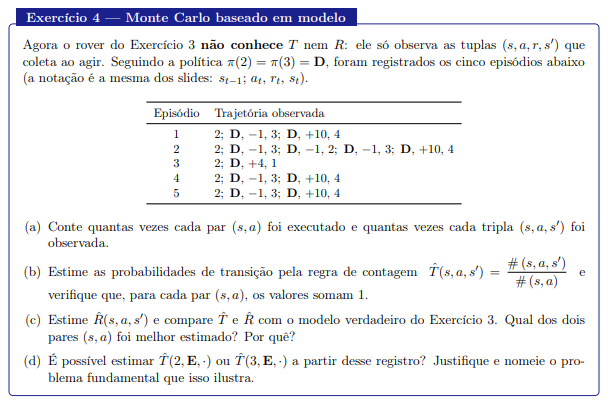
\includegraphics[width=0.8\textwidth]{ex4.png}
    \label{fig:ex4}
\end{figure}


\subsection{Item (a)}

Considerando os cinco episódios observados,
realizamos a contagem das execuções de cada
par estado-ação $(s,a)$ e das ocorrências
de cada transição $(s,a,s')$.

Como a política utilizada é
$\pi(2)=\pi(3)=D$, apenas a ação $D$
foi executada nos episódios.

\textbf{Contagem dos pares estado-ação:}

\begin{table}[H]
    \centering
    \caption{Número de execuções dos pares estado-ação}
    \label{tab:contagem_sa}
    \begin{tabular}{cc}
        \toprule
        Par $(s,a)$ & Número de execuções \\
        \midrule
        $(2,D)$ & 6 \\
        $(3,D)$ & 5 \\
        \midrule
        Total & 11 \\
        \bottomrule
    \end{tabular}
\end{table}

\textbf{Contagem das transições observadas:}

\begin{table}[H]
    \centering
    \caption{Número de ocorrências das transições}
    \label{tab:contagem_sas}
    \begin{tabular}{cccc}
        \toprule
        $s$ & $a$ & $s'$ & Ocorrências \\
        \midrule
        2 & D & 3 & 5 \\
        2 & D & 1 & 1 \\
        3 & D & 4 & 4 \\
        3 & D & 2 & 1 \\
        \bottomrule
    \end{tabular}
\end{table}

Para o par $(2,D)$, foram observadas
cinco transições para a célula $3$
e uma transição para a célula $1$:

\[
    \#(2,D)=5+1=6
\]

Para o par $(3,D)$, foram observadas
quatro transições para a célula $4$
e uma transição para a célula $2$:

\[
    \#(3,D)=4+1=5
\]

Portanto, foram registradas $11$
transições ao longo dos cinco episódios,
considerando todas as ocorrências,
inclusive as repetições dentro de um
mesmo episódio.


\subsection{Item (b)}

As probabilidades de transição são estimadas
pela frequência relativa das transições
observadas nos episódios.

A regra de contagem é definida por:

\[
    \hat{T}(s,a,s') =
    \frac{\#(s,a,s')}{\#(s,a)}
\]

em que $\#(s,a,s')$ representa o número
de ocorrências da transição $(s,a,s')$
e $\#(s,a)$ representa o número total
de execuções do par estado-ação.

\textbf{Transições a partir da célula 2:}

Como o par $(2,D)$ foi executado seis vezes,
sendo cinco transições para a célula $3$
e uma para a célula $1$, temos:

\[
\begin{aligned}
\hat{T}(2,D,3)
&=\frac{5}{6}\approx0{,}8333
\\[6pt]
\hat{T}(2,D,1)
&=\frac{1}{6}\approx0{,}1667
\end{aligned}
\]

\textbf{Transições a partir da célula 3:}

Como o par $(3,D)$ foi executado cinco vezes,
sendo quatro transições para a célula $4$
e uma para a célula $2$, temos:

\[
\begin{aligned}
\hat{T}(3,D,4)
&=\frac{4}{5}=0{,}8
\\[6pt]
\hat{T}(3,D,2)
&=\frac{1}{5}=0{,}2
\end{aligned}
\]

A Tabela~\ref{tab:probabilidades_estimadas}
apresenta as probabilidades estimadas.

\begin{table}[H]
    \centering
    \caption{Probabilidades de transição estimadas}
    \label{tab:probabilidades_estimadas}
    \begin{tabular}{cccc}
        \toprule
        $s$ & $a$ & $s'$ & $\hat{T}(s,a,s')$ \\
        \midrule
        2 & D & 3 & $\frac{5}{6}$ \\
        2 & D & 1 & $\frac{1}{6}$ \\
        3 & D & 4 & $\frac{4}{5}$ \\
        3 & D & 2 & $\frac{1}{5}$ \\
        \bottomrule
    \end{tabular}
\end{table}

\textbf{Verificação das probabilidades:}

Para o par $(2,D)$:

\[
\begin{aligned}
\sum_{s'\in S}\hat{T}(2,D,s')
&=\frac{5}{6}+\frac{1}{6}\\
&=1
\end{aligned}
\]

Para o par $(3,D)$:

\[
\begin{aligned}
\sum_{s'\in S}\hat{T}(3,D,s')
&=\frac{4}{5}+\frac{1}{5}\\
&=1
\end{aligned}
\]

Portanto, as probabilidades estimadas
formam distribuições válidas, pois
somam $1$ para cada par estado-ação
observado.


\subsection{Item (c)}

A recompensa estimada $\hat{R}(s,a,s')$
é obtida pela média das recompensas
observadas para cada transição $(s,a,s')$.

Assim:

\[
\hat{R}(s,a,s') =
\frac{
\sum_{i=1}^{\#(s,a,s')} r_i
}{
\#(s,a,s')
}
\]

em que $r_i$ representa a recompensa
observada em cada ocorrência da transição.

Como todas as ocorrências de uma mesma
transição apresentaram recompensas iguais,
obtemos:

\[
\begin{aligned}
\hat{R}(2,D,3)&=-1\\
\hat{R}(2,D,1)&=+4\\
\hat{R}(3,D,4)&=+10\\
\hat{R}(3,D,2)&=-1
\end{aligned}
\]

A Tabela~\ref{tab:comparacao_modelos}
apresenta a comparação entre as
probabilidades e recompensas estimadas
e os valores verdadeiros do Exercício 3.

\begin{table}[H]
\centering
\caption{Comparação entre o modelo estimado e o verdadeiro}
\label{tab:comparacao_modelos}
\begin{tabular}{ccccccc}
\toprule
$s$ & $a$ & $s'$ &
$T$ & $\hat{T}$ & $R$ & $\hat{R}$\\
\midrule
2 & D & 3 & $0{,}8$ & $\frac{5}{6}$ & $-1$ & $-1$\\
2 & D & 1 & $0{,}2$ & $\frac{1}{6}$ & $+4$ & $+4$\\
3 & D & 4 & $0{,}8$ & $\frac{4}{5}$ & $+10$ & $+10$\\
3 & D & 2 & $0{,}2$ & $\frac{1}{5}$ & $-1$ & $-1$\\
\bottomrule
\end{tabular}
\end{table}

Observa-se que todas as recompensas
foram estimadas exatamente:

\[
    \hat{R}(s,a,s')=R(s,a,s')
\]

para todas as transições observadas.

Entretanto, as probabilidades de transição
apresentam diferenças para o par $(2,D)$.

O erro absoluto das probabilidades
estimadas para esse par é:

\[
\begin{aligned}
\left|\frac{5}{6}-0{,}8\right|
&=\frac{1}{30}\approx0{,}0333
\\[6pt]
\left|\frac{1}{6}-0{,}2\right|
&=\frac{1}{30}\approx0{,}0333
\end{aligned}
\]

Já para o par $(3,D)$, as probabilidades
estimadas coincidem exatamente com
as probabilidades verdadeiras:

\[
\begin{aligned}
\hat{T}(3,D,4)&=T(3,D,4)=0{,}8\\
\hat{T}(3,D,2)&=T(3,D,2)=0{,}2
\end{aligned}
\]

Portanto, o par $(3,D)$ foi melhor
estimado nesta amostra, pois apresentou
erro nulo nas probabilidades de transição,
enquanto o par $(2,D)$ apresentou
pequenas diferenças.

Essa diferença decorre da variabilidade
aleatória das observações. Mesmo com
menos execuções, o par $(3,D)$ apresentou
frequências relativas iguais às
probabilidades verdadeiras.

Isso não significa que menos observações
produzam estimativas melhores, mas apenas
que, nesta amostra específica, os
resultados de $(3,D)$ coincidiram
com o modelo verdadeiro.


\subsection{Item (d)}

Não é possível estimar as probabilidades
de transição $\hat{T}(2,E,\cdot)$ e
$\hat{T}(3,E,\cdot)$ a partir dos
episódios fornecidos.

Isso ocorre porque todos os episódios
foram gerados seguindo a política:

\[
    \pi(2)=\pi(3)=D
\]

Portanto, a ação $E$ nunca foi executada
em nenhum dos estados observados.

Como a estimativa das probabilidades
depende das frequências observadas:

\[
    \hat{T}(s,a,s') =
    \frac{\#(s,a,s')}{\#(s,a)}
\]

para os pares $(2,E)$ e $(3,E)$,
temos:

\[
    \#(2,E)=\#(3,E)=0
\]

Consequentemente, o denominador da
expressão é zero, impossibilitando
o cálculo dessas estimativas.

Essa situação ilustra o problema
fundamental da
\textbf{exploração versus explotação}
(\textit{exploration vs. exploitation}).

A exploração consiste em experimentar
diferentes ações para obter informações
sobre o ambiente, enquanto a explotação
consiste em utilizar as ações consideradas
mais vantajosas com base no conhecimento
já adquirido.

Nesse caso, como o agente executou
exclusivamente a ação $D$, não coletou
informações suficientes para estimar
o comportamento da ação $E$.

Portanto, seria necessário explorar
também a ação $E$ para estimar
suas probabilidades de transição.

\section{Exercício 5}
\begin{figure}[H]
    \centering
    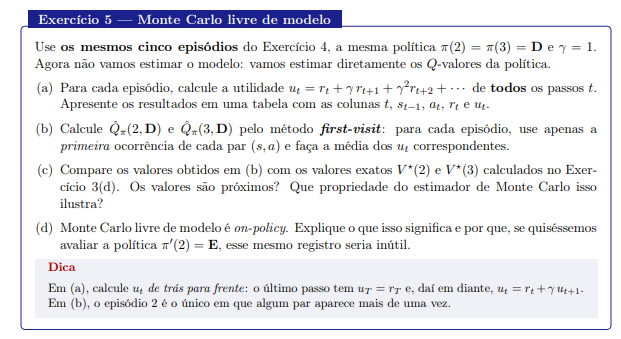
\includegraphics[width=0.8\textwidth]{ex5.png}
    \label{fig:ex5}
\end{figure}


\subsection{Item (a)}

No método de Monte Carlo livre de modelo,
a utilidade $u_t$ representa a soma
descontada das recompensas recebidas
a partir do passo $t$ até o final do episódio.

Sua expressão é dada por:

\[
    u_t = r_t + \gamma r_{t+1}
    + \gamma^2 r_{t+2} + \cdots
\]

Como o fator de desconto é $\gamma=1$,
a utilidade corresponde à soma de todas
as recompensas restantes:

\[
    u_t = \sum_{k=t}^{T} r_k
\]

em que $T$ representa o último passo
do episódio.

\textbf{Episódio 1:}

As recompensas observadas são $(-1,+10)$.

\[
\begin{aligned}
u_1 &= -1+10=9\\
u_2 &= 10
\end{aligned}
\]

\textbf{Episódio 2:}

As recompensas observadas são
$(-1,-1,-1,+10)$.

\[
\begin{aligned}
u_1 &= -1-1-1+10=7\\
u_2 &= -1-1+10=8\\
u_3 &= -1+10=9\\
u_4 &= 10
\end{aligned}
\]

\textbf{Episódio 3:}

O episódio possui apenas uma transição,
com recompensa $+4$.

\[
    u_1=4
\]

\textbf{Episódio 4:}

As recompensas observadas são $(-1,+10)$.

\[
\begin{aligned}
u_1 &= -1+10=9\\
u_2 &= 10
\end{aligned}
\]

\textbf{Episódio 5:}

As recompensas observadas são $(-1,+10)$.

\[
\begin{aligned}
u_1 &= -1+10=9\\
u_2 &= 10
\end{aligned}
\]

\textbf{Tabela de resultados:}

A Tabela~\ref{tab:utilidades_mc} apresenta
as utilidades calculadas para todos
os passos dos cinco episódios.

\begin{table}[H]
\centering
\caption{Utilidades dos episódios de Monte Carlo}
\label{tab:utilidades_mc}
\begin{tabular}{cccccc}
\toprule
Episódio & $t$ & $s_{t-1}$ & $a_t$ & $r_t$ & $u_t$\\
\midrule
1 & 1 & 2 & D & $-1$ & 9\\
1 & 2 & 3 & D & $+10$ & 10\\
\midrule
2 & 1 & 2 & D & $-1$ & 7\\
2 & 2 & 3 & D & $-1$ & 8\\
2 & 3 & 2 & D & $-1$ & 9\\
2 & 4 & 3 & D & $+10$ & 10\\
\midrule
3 & 1 & 2 & D & $+4$ & 4\\
\midrule
4 & 1 & 2 & D & $-1$ & 9\\
4 & 2 & 3 & D & $+10$ & 10\\
\midrule
5 & 1 & 2 & D & $-1$ & 9\\
5 & 2 & 3 & D & $+10$ & 10\\
\bottomrule
\end{tabular}
\end{table}

Portanto, as utilidades foram calculadas
considerando o retorno acumulado de cada
passo até o encerramento do respectivo episódio,
sem a necessidade de estimar as probabilidades
de transição do ambiente.


\subsection{Item (b)}

No método de Monte Carlo \textit{first-visit},
o Q-valor de um par estado-ação $(s,a)$
é estimado pela média das utilidades
observadas na primeira ocorrência desse
par em cada episódio.

A estimativa é dada por:

\[
\hat{Q}_{\pi}(s,a)=
\frac{1}{N(s,a)}
\sum_{i=1}^{N(s,a)}u_i(s,a)
\]

em que $N(s,a)$ representa o número de
episódios nos quais o par $(s,a)$ foi
visitado, e $u_i(s,a)$ é a utilidade
de sua primeira ocorrência no episódio $i$.

A Tabela~\ref{tab:first_visit} apresenta
as utilidades consideradas para cada par.

\begin{table}[H]
\centering
\caption{Utilidades consideradas no método first-visit}
\label{tab:first_visit}
\begin{tabular}{ccc}
\toprule
Episódio & $(2,D)$ & $(3,D)$\\
\midrule
1 & 9 & 10\\
2 & 7 & 8\\
3 & 4 & --\\
4 & 9 & 10\\
5 & 9 & 10\\
\bottomrule
\end{tabular}
\end{table}

\textbf{Estimativa de $\hat{Q}_{\pi}(2,D)$:}

O par $(2,D)$ aparece nos cinco episódios.
Considerando apenas sua primeira ocorrência
em cada um deles, temos:

\[
\begin{aligned}
\hat{Q}_{\pi}(2,D)
&=\frac{9+7+4+9+9}{5}\\
&=\frac{38}{5}\\
&=7{,}6
\end{aligned}
\]

Portanto:

\[
\boxed{\hat{Q}_{\pi}(2,D)=7{,}6}
\]

\textbf{Estimativa de $\hat{Q}_{\pi}(3,D)$:}

O par $(3,D)$ aparece em quatro episódios,
não sendo observado no episódio $3$.

Considerando apenas a primeira ocorrência
em cada episódio:

\[
\begin{aligned}
\hat{Q}_{\pi}(3,D)
&=\frac{10+8+10+10}{4}\\
&=\frac{38}{4}\\
&=9{,}5
\end{aligned}
\]

Portanto:

\[
\boxed{\hat{Q}_{\pi}(3,D)=9{,}5}
\]

No episódio $2$, os pares $(2,D)$ e $(3,D)$
aparecem mais de uma vez. Entretanto,
pelo critério \textit{first-visit},
somente as utilidades da primeira ocorrência
de cada par são utilizadas.

Assim, os Q-valores estimados são:

\[
\boxed{
\begin{aligned}
\hat{Q}_{\pi}(2,D)&=7{,}6\\
\hat{Q}_{\pi}(3,D)&=9{,}5
\end{aligned}
}
\]


\subsection{Item (c)}

No Exercício 3(d), foram obtidos os
valores ótimos exatos:

\[
\begin{aligned}
V^\star(2)&=\frac{52}{7}\approx7{,}4286\\
V^\star(3)&=\frac{65}{7}\approx9{,}2857
\end{aligned}
\]

No item (b), utilizando o método de
Monte Carlo \textit{first-visit},
obtivemos as estimativas:

\[
\begin{aligned}
\hat{Q}_{\pi}(2,D)&=7{,}6\\
\hat{Q}_{\pi}(3,D)&=9{,}5
\end{aligned}
\]

Como a política utilizada é
$\pi(2)=\pi(3)=D$, que corresponde
à política ótima encontrada no
Exercício 3, podemos comparar
diretamente essas estimativas com
os valores ótimos exatos.

\textbf{Cálculo dos erros absolutos:}

Para o estado $2$:

\[
\begin{aligned}
E_2
&=\left|7{,}6-\frac{52}{7}\right|\\
&=\frac{6}{35}\\
&\approx0{,}1714
\end{aligned}
\]

Para o estado $3$:

\[
\begin{aligned}
E_3
&=\left|9{,}5-\frac{65}{7}\right|\\
&=\frac{3}{14}\\
&\approx0{,}2143
\end{aligned}
\]

A Tabela~\ref{tab:comparacao_mc}
apresenta os resultados.

\begin{table}[H]
\centering
\caption{Comparação entre os valores exatos e estimados}
\label{tab:comparacao_mc}
\begin{tabular}{cccc}
\toprule
Estado & Valor exato & Estimativa MC & Erro absoluto\\
\midrule
2 & $7{,}4286$ & $7{,}6000$ & $0{,}1714$\\
3 & $9{,}2857$ & $9{,}5000$ & $0{,}2143$\\
\bottomrule
\end{tabular}
\end{table}

Observa-se que as estimativas de Monte Carlo
são próximas dos valores exatos, mesmo
utilizando apenas cinco episódios.

As pequenas diferenças decorrem da
variabilidade aleatória das trajetórias
observadas.

Esse resultado ilustra a propriedade de
\textbf{consistência do estimador de
Monte Carlo}.

À medida que o número de episódios
independentes aumenta, a média das
utilidades observadas tende a convergir
para o valor esperado verdadeiro
da política avaliada, conforme
a Lei dos Grandes Números.

Portanto, embora as estimativas possam
apresentar erros com poucas observações,
elas tendem a se tornar mais precisas
com o aumento da quantidade de episódios.


\subsection{Item (d)}

O método de Monte Carlo livre de modelo
utilizado é classificado como
\textit{on-policy}, pois a política
avaliada é a mesma utilizada para
gerar os episódios de experiência.

Nesse método, os Q-valores são
estimados a partir das recompensas
acumuladas em trajetórias produzidas
pela própria política $\pi$.

No exercício, todos os episódios
foram gerados seguindo a política:

\[
    \pi(2)=\pi(3)=D
\]

Portanto, as estimativas obtidas
correspondem aos Q-valores dessa política.

Entretanto, caso desejássemos avaliar
uma política alternativa $\pi'$,
definida por:

\[
    \pi'(2)=E
\]

o mesmo registro não seria suficiente,
pois a ação $E$ nunca foi executada
na célula $2$.

Consequentemente, não existem
observações do par $(2,E)$:

\[
    \#(2,E)=0
\]

Além disso, os retornos observados
após executar a ação $D$ não representam
diretamente os retornos que seriam
obtidos seguindo a política $\pi'$.

Assim, seria necessário gerar novos
episódios seguindo a política $\pi'$
para avaliá-la diretamente pelo
método Monte Carlo \textit{on-policy}.

Essa limitação evidencia a dependência
do método em relação à política
utilizada na coleta dos dados.

Métodos \textit{off-policy}, por outro
lado, permitem avaliar uma política
diferente daquela utilizada para
gerar os episódios, desde que
sejam atendidas as condições necessárias
para essa avaliação.

\section{Exercício 6}
\begin{figure}[H]
    \centering
    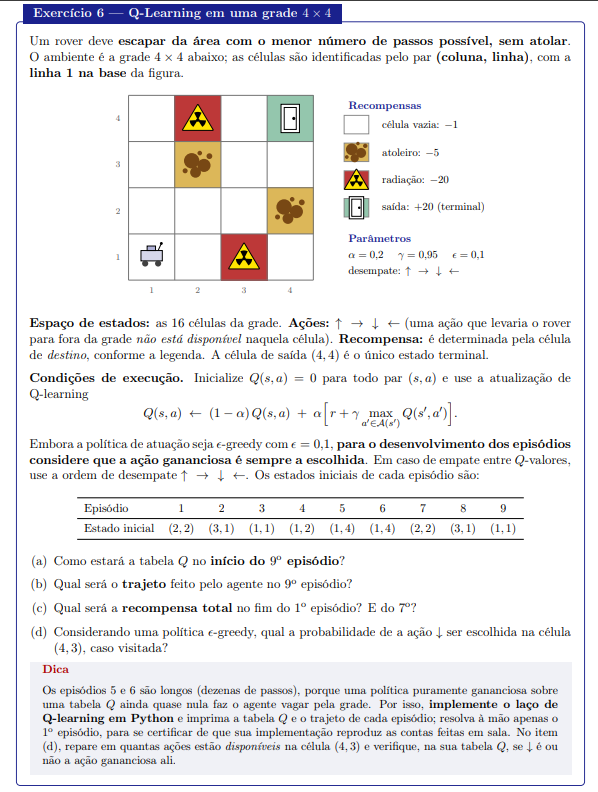
\includegraphics[width=0.8\textwidth]{ex6.png}
    \label{fig:ex6}
\end{figure}


\subsection{Item (a)}

Para determinar a tabela $Q$ no início
do nono episódio, executamos o algoritmo
Q-Learning durante os oito primeiros
episódios, utilizando os parâmetros:

\[
\alpha=0{,}2,\qquad
\gamma=0{,}95,\qquad
\epsilon=0{,}1
\]

Inicialmente, todos os Q-valores são
iguais a zero:

\[
Q(s,a)=0,\quad \forall(s,a)
\]

Conforme solicitado, durante a execução
dos episódios a ação escolhida é sempre
a gananciosa, com desempate na ordem:

\[
\uparrow\;,\quad
\rightarrow\;,\quad
\downarrow\;,\quad
\leftarrow
\]

A atualização utilizada é:

\[
Q(s,a)\leftarrow
(1-\alpha)Q(s,a)+
\alpha\left[
r+\gamma\max_{a'\in A(s')}Q(s',a')
\right]
\]

Substituindo os parâmetros:

\[
Q(s,a)\leftarrow
0{,}8Q(s,a)+
0{,}2\left[
r+0{,}95\max_{a'\in A(s')}Q(s',a')
\right]
\]

Nos estados terminais, o valor
das recompensas futuras é zero.

\textbf{Resultados dos oito episódios:}

\begin{table}[H]
\centering
\caption{Execução dos oito primeiros episódios}
\label{tab:episodios_qlearning}
\begin{tabular}{ccc}
\toprule
Episódio & Número de passos & Recompensa total\\
\midrule
1 & 4  & $-6$\\
2 & 4  & $+17$\\
3 & 8  & $-10$\\
4 & 5  & $+12$\\
5 & 39 & $-83$\\
6 & 23 & $-2$\\
7 & 10 & $+11$\\
8 & 6  & $+11$\\
\bottomrule
\end{tabular}
\end{table}

\textbf{Tabela Q no início do nono episódio:}

A Tabela~\ref{tab:q_inicio_ep9} apresenta
os Q-valores obtidos após a execução
dos oito episódios, arredondados
para quatro casas decimais.

\begin{table}[H]
\centering
\small
\caption{Tabela Q no início do nono episódio}
\label{tab:q_inicio_ep9}
\begin{tabular}{ccccc}
\toprule
Estado $(x,y)$ &
$Q(s,\uparrow)$ &
$Q(s,\rightarrow)$ &
$Q(s,\downarrow)$ &
$Q(s,\leftarrow)$\\
\midrule
$(1,1)$ & $-0{,}9563$ & $-0{,}7927$ & -- & --\\
$(2,1)$ & $-0{,}7752$ & $-4{,}0000$ & -- & $-0{,}8936$\\
$(3,1)$ & $-0{,}3600$ & $-0{,}5500$ & -- & $-0{,}2000$\\
$(4,1)$ & $-1{,}8000$ & -- & -- & $-4{,}0000$\\
\midrule
$(1,2)$ & $-0{,}9505$ & $-0{,}9159$ & $-0{,}7903$ & --\\
$(2,2)$ & $-1{,}0000$ & $-0{,}6443$ & $-0{,}8156$ & $-0{,}6315$\\
$(3,2)$ & $1{,}6287$ & $-1{,}0000$ & $-4{,}0380$ & $-0{,}2380$\\
$(4,2)$ & $-0{,}2000$ & -- & $-0{,}2000$ & $-0{,}0308$\\
\midrule
$(1,3)$ & $-0{,}8519$ & $-1{,}0000$ & $-1{,}0058$ & --\\
$(2,3)$ & $-4{,}0000$ & $-0{,}0936$ & $-0{,}2000$ & $0{,}0000$\\
$(3,3)$ & $7{,}3045$ & $0{,}0000$ & $0{,}0000$ & $0{,}0000$\\
$(4,3)$ & $4{,}0000$ & -- & $0{,}0000$ & $0{,}0000$\\
\midrule
$(1,4)$ & -- & $-4{,}0000$ & $-0{,}9379$ & --\\
$(2,4)$ & -- & $-0{,}2000$ & $-1{,}0000$ & $0{,}0000$\\
$(3,4)$ & -- & $15{,}8057$ & $0{,}0000$ & $0{,}0000$\\
$(4,4)$ & -- & -- & -- & --\\
\bottomrule
\end{tabular}
\end{table}

Na tabela, o símbolo ``--'' indica
uma ação indisponível naquela célula.
O estado $(4,4)$ é terminal e,
portanto, não possui ações disponíveis.

Os valores iguais a zero correspondem
a ações que ainda não receberam
atualizações durante os episódios.

Observa-se que os maiores Q-valores
estão próximos da saída $(4,4)$,
especialmente nos estados $(3,4)$
e $(3,3)$.

Isso ocorre porque o agente
passa a incorporar às estimativas
as recompensas positivas associadas
à chegada ao estado terminal.


\subsection{Item (b)}

O nono episódio inicia no estado $(1,1)$,
utilizando a tabela $Q$ obtida após
os oito primeiros episódios.

Em cada passo, o agente seleciona
a ação com maior Q-valor disponível:

\[
a_t=\arg\max_{a\in A(s_t)}Q(s_t,a)
\]

Em caso de empate, utiliza-se
a ordem de prioridade:

\[
\uparrow,\quad\rightarrow,\quad
\downarrow,\quad\leftarrow
\]

A Tabela~\ref{tab:trajeto_ep9} apresenta
a sequência de movimentos realizada
pelo agente.

\begin{table}[H]
\centering
\caption{Trajeto do agente no nono episódio}
\label{tab:trajeto_ep9}
\begin{tabular}{ccccc}
\toprule
Passo & Estado & Ação & Próximo estado & Recompensa\\
\midrule
1 & $(1,1)$ & $\rightarrow$ & $(2,1)$ & $-1$\\
2 & $(2,1)$ & $\uparrow$ & $(2,2)$ & $-1$\\
3 & $(2,2)$ & $\leftarrow$ & $(1,2)$ & $-1$\\
4 & $(1,2)$ & $\downarrow$ & $(1,1)$ & $-1$\\
5 & $(1,1)$ & $\uparrow$ & $(1,2)$ & $-1$\\
6 & $(1,2)$ & $\rightarrow$ & $(2,2)$ & $-1$\\
7 & $(2,2)$ & $\rightarrow$ & $(3,2)$ & $-1$\\
8 & $(3,2)$ & $\uparrow$ & $(3,3)$ & $-1$\\
9 & $(3,3)$ & $\uparrow$ & $(3,4)$ & $-1$\\
10 & $(3,4)$ & $\rightarrow$ & $(4,4)$ & $+20$\\
\bottomrule
\end{tabular}
\end{table}

O trajeto completo é:

\[
\begin{aligned}
(1,1)&\rightarrow(2,1)\rightarrow(2,2)\\
&\rightarrow(1,2)\rightarrow(1,1)\\
&\rightarrow(1,2)\rightarrow(2,2)\\
&\rightarrow(3,2)\rightarrow(3,3)\\
&\rightarrow(3,4)\rightarrow(4,4)
\end{aligned}
\]

O agente realiza dez movimentos até
alcançar a saída $(4,4)$.

Durante o percurso, passa apenas por
células vazias, recebendo nove
penalidades de $-1$ e a recompensa
terminal de $+20$.

Assim, a recompensa total do episódio é:

\[
R_{\text{total}}=9(-1)+20
\]

\[
\boxed{R_{\text{total}}=11}
\]

Observa-se que o agente ainda realiza
movimentos desnecessários, retornando
a estados anteriormente visitados.

Isso ocorre porque a tabela $Q$
ainda não convergiu para os valores
ótimos, fazendo com que a política
gananciosa apresente decisões
subótimas durante o percurso.


\subsection{Item (c)}

A recompensa total de cada episódio é
calculada pela soma das recompensas
recebidas em todas as transições
até alcançar o estado terminal.

\[
R_{\text{total}}=\sum_{t=1}^{T}r_t
\]

\textbf{Episódio 1:}

O agente parte do estado $(2,2)$
e realiza o seguinte trajeto:

\[
\begin{aligned}
(2,2)&\rightarrow(2,3)\rightarrow(2,4)\\
&\rightarrow(3,4)\rightarrow(4,4)
\end{aligned}
\]

As recompensas recebidas são:

\begin{itemize}
    \item $(2,3)$: atoleiro, recompensa $-5$;
    \item $(2,4)$: radiação, recompensa $-20$;
    \item $(3,4)$: célula vazia, recompensa $-1$;
    \item $(4,4)$: saída, recompensa $+20$.
\end{itemize}

Assim:

\[
\begin{aligned}
R_{\text{total}}^{(1)}
&=-5-20-1+20\\
&=-6
\end{aligned}
\]

Portanto:

\[
\boxed{R_{\text{total}}^{(1)}=-6}
\]

\textbf{Episódio 7:}

O agente parte novamente do estado $(2,2)$
e realiza o trajeto:

\[
\begin{aligned}
(2,2)&\rightarrow(2,1)\rightarrow(1,1)\\
&\rightarrow(1,2)\rightarrow(1,3)\\
&\rightarrow(1,2)\rightarrow(2,2)\\
&\rightarrow(3,2)\rightarrow(3,3)\\
&\rightarrow(3,4)\rightarrow(4,4)
\end{aligned}
\]

Nesse episódio, o agente realiza dez
movimentos, sendo nove transições para
células vazias, com recompensa $-1$,
e uma transição para a saída, com
recompensa $+20$.

Logo:

\[
\begin{aligned}
R_{\text{total}}^{(7)}
&=9(-1)+20\\
&=-9+20\\
&=11
\end{aligned}
\]

Portanto:

\[
\boxed{R_{\text{total}}^{(7)}=11}
\]

\textbf{Comparação dos resultados:}

\[
\begin{aligned}
R_{\text{total}}^{(1)}&=-6\\
R_{\text{total}}^{(7)}&=11
\end{aligned}
\]

A diferença entre as recompensas é:

\[
\Delta R=11-(-6)=17
\]

Assim, o episódio 7 apresenta uma
recompensa total 17 unidades maior
que o episódio 1.

Essa melhoria ocorre porque, após
as atualizações da tabela $Q$,
o agente passa a evitar as células
com maiores penalidades.

Embora o trajeto do episódio 7
seja mais longo, ele produz uma
recompensa total superior por
evitar o atoleiro e a radiação.


\subsection{Item (d)}

Na política $\epsilon$-greedy, o agente
seleciona a ação gananciosa com
probabilidade $1-\epsilon$ e realiza
uma escolha aleatória entre as ações
disponíveis com probabilidade $\epsilon$.

Considerando $\epsilon=0{,}1$,
analisamos o estado $(4,3)$.

Nessa célula, as ações disponíveis são:

\[
A((4,3))=
\{\uparrow,\downarrow,\leftarrow\}
\]

A ação $\rightarrow$ não está disponível,
pois levaria o agente para fora da grade.

Conforme a tabela $Q$ obtida no item (a):

\[
\begin{aligned}
Q((4,3),\uparrow)&=4\\
Q((4,3),\downarrow)&=0\\
Q((4,3),\leftarrow)&=0
\end{aligned}
\]

Portanto, a ação gananciosa é:

\[
a^\star=\uparrow
\]

Como a ação $\downarrow$ não é gananciosa,
ela somente pode ser selecionada
durante a exploração aleatória.

Na definição de $\epsilon$-greedy em que
a exploração sorteia uniformemente entre
todas as ações disponíveis, temos:

\[
P(\downarrow\mid(4,3))
=\frac{\epsilon}{|A((4,3))|}
\]

Substituindo os valores:

\[
\begin{aligned}
P(\downarrow\mid(4,3))
&=\frac{0{,}1}{3}\\
&\approx0{,}0333
\end{aligned}
\]

Portanto:

\[
\boxed{
P(\downarrow\mid(4,3))\approx3{,}33\%
}
\]

Assim, a probabilidade de escolher
a ação $\downarrow$ na célula $(4,3)$
é aproximadamente $3{,}33\%$.
